% ВАЖНО
% Не меняйте ничего в этом файле. А если меняете, то делайте это в этом проекте:
% https://github.com/kib-courses/latex_templates
% Для пользовательских настроек есть файл ./header/user.tex
\documentclass{beamer}
\usetheme{metropolis} 
\usecolortheme{rose}

\hypersetup{unicode=true}
\usepackage{tikz}

\usepackage{xcolor}
\usepackage[utf8]{inputenc}
\usepackage{hyphenat}
\usepackage[russian,english]{babel}          % Use metropolis theme
\usepackage{wrapfig}

\usepackage[normalem]{ulem}  % для зачекивания текста

\usepackage{caption}
\captionsetup[figure]{name=Рисунок }
\newcommand{\рис}[1]{рис.\ref{#1}}
\newcommand{\Рис}[1]{Рис.\ref{#1}}


\captionsetup[table]{name=Таблица~№}
\newcommand{\таблицa}[1]{таблица~№\ref{#1}} % именительный падеж
\newcommand{\таблицы}[1]{таблицы~№\ref{#1}} % родительный падеж
\newcommand{\таблице}[1]{таблице~№\ref{#1}} % дательный и предложный падеж
\newcommand{\таблицу}[1]{таблицу~№\ref{#1}} % винительный падеж
\newcommand{\таблицей}[1]{таблицей~№\ref{#1}} % творительный падеж 
\newcommand{\Таблицa}[1]{Таблица~№\ref{#1}} % именительный падеж
\newcommand{\Таблицы}[1]{Таблицы~№\ref{#1}} % родительный падеж
\newcommand{\Таблице}[1]{Таблице~№\ref{#1}} % дательный и предложный падеж
\newcommand{\Таблицу}[1]{Таблицу~№\ref{#1}} % винительный падеж
\newcommand{\Таблицей}[1]{Таблицей~№\ref{#1}} % творительный падеж 

\setbeamertemplate{footline}[frame number] % указывает на каждой странице общее количество страниц

% Указывайте все новые термины в \termdef команде. А уже известные ранее или из других курсов в \term
\newcommand{\termdef}[1]{\textbf{\textit{#1}}}
\newcommand{\term}{\textit}

% Диалог с аудиторией.
\newcommand{\auditorium}[1]{\textcolor{red}{\textbf{#1}}}

% Вопрос к аудитории 
\newcommand{\вопрос}[1]{\textbf{\textcolor{red}{#1}}}
\newcommand{\внекурса}[1]{\textbf{\textcolor{violet}{#1}}}
\newcommand{\дз}[1]{\textbf{\textcolor{teal}{#1}}}  

% TODO ! напишите здесь название вашей лекции
\title{Лекция 1. Комбинаторика часть 1.}
% TODO ! замените на дату проведения этой лекции. Например \date{14 апреля 2019}
\date{<TODO дата>}
% \logo{\href{https://t.me/kibinfo}{
\includegraphics[width=.05\textwidth]{./../pic/kib_logo.png}}}
\author{Слипенчук Павел Владимирович}
\institute{\centering 
\includegraphics[width=.2\textwidth]{./../pic/kib_logo.png} \\ Москва,\\ \href{https://t.me/kibinfo}{\textbf{КИБ}} }
% \titlegraphic{\href{https://t.me/kibinfo}{
\includegraphics[width=.05\textwidth]{./../pic/kib_logo.png}}}

% TODO ! замените https://github.com/kib-courses/latex_templates на ссылку ВАШЕГО спецкурса!
\titlegraphic{\small \href{https://github.com/kib-courses/dsis-math-base}{Базовая математическая подготовка для Data Science}}

\begin{document}
  \maketitle
    
  \begin{frame}{План лекции}\label{frame:plan}
  	% TODO ! добавте в план все ваши секции, кроме "Вопросы для самопроверки", "Домашнее задание" и "Список материалов"
    \begin{enumerate}
	\item \nameref{section:why_combinatorics}
	\item \nameref{section:principles}
	\item \nameref{section:main_combinatorics_sxems}
	\item \nameref{section:binom}
	% \item \nameref{section:tkiz}
	% \item \nameref{section:another}
	\end{enumerate}
 \end{frame}
    
\section{Зачем нужна комбинаторика в DS}\label{section:why_combinatorics}
\begin{frame}
\termdef{Комбинаторный анализ (Комбинаторика)} — раздел математики, посвящённый 
решению задач выбора и расположения элементов некоторого, обычно конечного, множества
в соответствии с установленными правилами (схемами). 

Каждое такое правило определяет способ построения из элементов исходного множества некоторой конструкции, 
называемой \termdef{комбинаторной конфигурацией}. 
\end{frame}


\begin{frame}{Примеры задач комбинаторики}

\textbf{Простая задача.}
В школе танго 8 парней 
и 12 девушек.
Сколько существует всевозможных пар?

\begin{equation*}
8 \cdot 12 = 96
\end{equation*}

\textbf{Сложная задача.}
Сколько потребуется бит данных, 
чтобы сохранить всевозможные первые 20 ходов в шахматах?
\end{frame}


\begin{frame}{<<Задача о зёрнах на шахматной доске>>}
	
	\textbf{Когда очень много кажется малым...}
	
	Согласно индийской легенде, 
	брахман Сисса придумал шахматы (чатурангу).
	Правителю так понравилась игра, что он предложил Сиссе 
	выбрать себе награду.
	
	Хитрый Сисса попросил у правителя 
	на первую клетку положить одно зёрнышко пшеницы,
	на вторую два, 
	на третью четыре,
	на пятую восемь и так далее.
	
	Правитель, не разбиравшийся в комбинаторике,
	быстро согласился, даже несколько 
	обидевшись на столь "невысокую" цену.
	
	Однако неделю спустя 
	казначей доложил правителю что расплатиться невозможно,
	"разве что осушить моря и океаны и засеять всё пшеницей".
	
\end{frame}

\begin{frame}{<<Задача о зёрнах на шахматной доске>>}

\begin{equation*}
\begin{matrix}
C = 1 + 2 + 4 + 8 + 16 + ... + 2^{63} = \sum_{i=0}^{i=63} 2^i = 2^{64} - 1 = \\
= 18~446~744~073~709~551~615
\end{matrix}
\end{equation*}

Много или мало $2^{64}$ зёрен пшеницы ?

В 2021 году было произведено в мире 770 млн.тонн пшеницы.
Вес одного зерна примерно $50$ милиграмм.

\дз{Вопрос: сколько тысячелетий люди должны перестать есть хлеб, чтобы Сисса получил 
свою оплату?} :)

\end{frame}

\begin{frame}
Задач, аналогичной классической 
<<Задаче о зёрнах...>>
в сфере Data Science чрезвычайно много.

Одна из целей комбинаторики:
понимать что такое МНОГО, ОЧЕНЬ МНОГО.

Например:
\begin{enumerate}
	\item ~<<Давайте мониторить все видео на youtube с целью проверки на стеганографию!>>
	\item ~<<ChatGPT скоро научиться отвечать на все вопросы!>>
\end{enumerate}
 	
\end{frame}


\begin{frame}
	Road Map Data Science как мат.дисциплины \(кратко\)
	\begin{center}
		\begin{figure}
			\begin{tikzpicture}[node distance=1.5cm,auto]
\tikzstyle{recfill}=[draw, fill=blue!10, minimum size=2em]
\tikzstyle{rect}=[draw,minimum size=2em]
\tikzstyle{inv}=[draw,minimum size=2em]
% \tikzstyle{init} = [pin edge={to-,thin,black}]
\node (c) [recfill] {Комбинаторика};
\node (s) [below of=c, rect] {Мат.стат.};
\node (p) [left of=s, node distance=3.5cm, rect] {Теор.вер.};
\node (a) [right of=s, node distance=3.5cm, rect] {\small Алгоритмы и с.д.};
\node (m) [below of=p,rect] {Мат.ан.};
\node (l) [below of=s, rect] {Лин.ал.};
\node (inv) [below of=a] {};
\node (ml) [below of=inv, rect] {\small Machine Learning};

\path[->] (c) edge node {} (p);
\path[->] (c) edge node {} (a);
\path[->] (p) edge node {} (s);
\path[->] (m) edge node {} (s);
\path[->] (s) edge node {} (a);
\path[->] (m) edge node {} (a);
\path[->] (m) edge node {} (p);
\path[->] (m) edge node {} (l);
\path[->] (l) edge node {} (ml);
\path[->] (s) edge node {} (ml);
\path[->] (a) edge node {} (ml);

\node (sa) [below of=l, rect] {\small Предметная область};
\node (ca) [below of=m, rect] {\small Computer Science};

\node (ds) [below of=sa, rect] {\small Data Science};

\path[->] (ml) edge node {} (ds);
\path[->] (sa) edge node {} (ds);
\path[->] (ca) edge node {} (ds);

% \node [int, pin={[init]above:$v_0$}] (a) {$\frac{1}{s}$};
% \node (b) [left of=a,node distance=2cm, coordinate] {a};
% \node [int, pin={[init]above:$p_0$}] (c) [right of=a] {$\frac{1}{s}$};
% \node [coordinate] (end) [right of=c, node distance=2cm]{};
% \path[->] (b) edge node {$a$} (a);
% \path[->] (a) edge node {$v$} (c);
% \draw[->] (c) edge node {$p$} (end) ;
\end{tikzpicture}


			\caption{Место комбинаторики в DS}
		\end{figure}	
	\end{center}
	
\end{frame}

\section{Комбинаторные принципы}\label{section:principles}

\begin{frame}{Два основных правила}
\termdef{Правило суммы. (Правило <<ИЛИ>>)}
Если элемент $A$ можно выбрать $a$ способами,
а элемент $B$ можно выбрать $b$ способами,
то выбрать $A$ или $B$ 
можно $a+b$ способами.

\termdef{Правило умножения. (Правило <<И>>)}
Если элемент $A$ можно выбрать $a$ способами,
а элемент $B$ можно выбрать $b$ способами,
то пару $(A, B)$ 
можно выбрать $a \cdot b$ способами.

\end{frame}

\begin{frame}{Формула включения-исключения}

%\termdef{Формула включения-исключения}

Посчитаем мощность множества (количество элементов в множестве)
вида $\left| A \cup B \right|$

\begin{equation}
\left| A \cup B \right| = \left|  A \right| + \left|  B \right| - \left| A \cap B \right|
\end{equation}

%\begin{wrapfigure}{r}{2cm}
\centering
	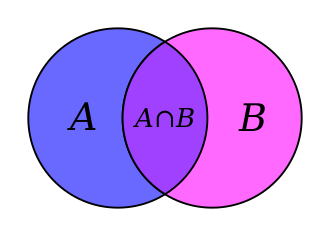
\includegraphics[width=2cm]{../pic/A_intersect_B.svg.png}
%	\caption{Круги Эйлера для формулы включения-исключения}
%	\label{figure:pelican_1}
%\end{wrapfigure}

\end{frame}

\begin{frame}{Принцип Дирихле}
<<Если кролики рассажены в клетки и число кроликов больше числа клеток, то хотя бы в одной из клеток находится более одного кролика.>>

<<Если число клеток больше числа кроликов, то как минимум одна клетка пуста.>>
\end{frame}

\begin{frame}{Out of scope}

Ряд комбинаторных вещей мы не рассматриваем:
\begin{enumerate}
	\item биективное доказателство; 
	\item производящие функции;
	\item рекуррентные соотношения.
\end{enumerate}

\внекурса{Самостоятельно 
их освойте после прохождения DSIS направления.}
\end{frame}


\section{Основные комбинаторные схемы}\label{section:main_combinatorics_sxems}


\begin{frame}{Размещение (выборка без возвращения)}
Нужно из
$n$
различных элементов 
выбрать \textbf{упорядоченный}
ряд из $k$
элементов. 
Элементы берутся не более одного раза.

(Согласно принципу Дирихле, очевидно, что $k \leqslant n$,
иначе задача не имеет решения.)


Сколько существует таких способов?   

Пример.
Есть $n$ различных действий для атаки.
Сколько существует вариантов сделать атаку из $k$ действий?

\begin{equation}
A_n^k = n \cdot (n-1) \cdot (n-2) \cdot ... \cdot (n-k-1) = \frac{n!} {\left(n-k\right)!}
\end{equation}    

\вопрос{Как вывести эту формулу?}

\end{frame}

\begin{frame}


\дз{Докажите строго формулу:}
\begin{equation}
A_n^k = n \cdot (n-1) \cdot (n-2) \cdot ... \cdot (n-k-1)
\end{equation}  

Подсказка: используйте правило умножения, здравый смысл 
и метод математической индукции

\end{frame}



\begin{frame}{Перестановка}
\termdef{Перестановка} -- 
частный случай \term{размещения}, 
когда $n=k$ 

\begin{equation}
P_n = A_n^n
\end{equation}

Пример. Сколько существует способ в шифротексте из $n$ блоков переставить эти блоки?
\end{frame}


\begin{frame}{Размещение с повторением}
Нужно из
$n$
различных элементов 
выбрать \textbf{упорядоченный}
ряд из $k$
элементов. 
При этом элементы можно выбирать более одного раза.

\begin{equation}
\overline{A}_n^k = n ^ k
\end{equation} 
\дз{выведите эту формулу.}

\end{frame}

\begin{frame}{Сочетание}
	
Нужно из
$n$
различных элементов 
выбрать \textbf{не упорядоченный}
ряд из $k$
элементов. 
Элементы берутся не более одного раза.

\begin{equation}
C_n^k = \frac{n!}{\left( n-k\right)! k!}
\end{equation}

Давайте выведем эту формулу

...
\end{frame}

\begin{frame}{Сочетание}

$C_n^k$ это то же самое, 
что и $A_n^k$, за исключением того, что порядок НЕ важен.
Значит если  $A_n^k$ умножить на число перестановок $P_k$,
то согласно правилу умножения получим $C_n^k$

Значит:
\begin{equation*}
A_n^k = C_n^k \cdot P_k = C_n^k \cdot A_k^k
\end{equation*}
следовательно верно:
\begin{equation*}
C_n^k = \frac{A_n^k}{A_k^k}
\end{equation*}

Далее нужно расписать формулу. 
\дз{сделайте это дома.}

\end{frame}

\begin{frame}{Сочетание с повторением}
Нужно из
$n$
различных элементов 
выбрать \textbf{не упорядоченный}
ряд из $k$
элементов.
При этом элементы можно брать более одного раза.

\begin{equation}
\overline{C}_n^k = C_{n+k-1}^{n-1}
\end{equation}

\дз{Попробуйте доказать это самостоятельно, используя подсказку из методички Жуковых на стр.6}
Если не получиться -- на ближайшем очном занятии распишем.
	
\end{frame}

\begin{frame}{Out of scope}
	
Мы не рассматриваем числа стирлинга 1-го и 2-го родов.

\внекурса{Самостоятельно 
		их освойте после прохождения DSIS направления.}
\end{frame}

\section{Бином Ньютона}\label{section:binom}

\begin{frame}

Бином Ньютона:
\begin{equation}\label{eq:binom}
\left( x + y\right)^n = \sum_{k=0}^{k=n} C_n^k \cdot x^{n-k} \cdot y^{k}
\end{equation}

Доказательство
\begin{equation*}
\begin{matrix}
\left( x + y\right)^2 = x^2 + 2xy + y^2 = C_{2}^0 x^2 y^0 + C_{2}^{1} xy + C_{2}^{2}x^0y^2 \\
\left( x + y\right)^3 = x^3 + 3x^2y + 3xy^2 + y^3 = C_{3}^{0}x^3y^0 + C_{3}^{1}x^2y + C_{3}^{2}xy^2 + C_{3}^{3}x^0y^3  
\end{matrix}
\end{equation*}

\дз{дома самостоятельно распишите $\left( x + y\right)^4$ и $\left( x + y\right)^5$}

База индукции есть.

Предположим, что верно 
\begin{equation}\label{eq:binom_prev}
\left( x + y\right)^(n-1) = \sum_{k=0}^{k=n-1} C_{(n-1)}^k \cdot x^{n-1-k} \cdot y^{k}
\end{equation}
тогда нужно из формулы \eqref{eq:binom_prev}
вывести формулу \eqref{eq:binom}

\дз{сделайте это!}
\end{frame}

\begin{frame}
Бином Ньютона полезен для доказательства разных формул.	

Например подставим $x=1$ и $y=1$ в формулу \eqref{eq:binom}.
Получим:
\begin{equation}
\begin{matrix}
(1+1)^n = \sum_{k=0}^{k=n} C_n^k \cdot 1^{n-k} \cdot 1^{k} \\
2^n = \sum_{k=0}^{k=n} C_n^k
\end{matrix}
\end{equation}


\end{frame}


%\section{Вопросы для самопроверки}

% \begin{frame}
% TODO
% \end{frame}

\section{Домашняя работа}
\begin{frame}

\small
\begin{enumerate}
 \item заведите толстую тетрадь в клетку, удобную ручку и маркеры.
 \item прочитайте ещё раз лекцию. Перепишите формулы.
 \item задания, выделенные \дз{этим цветом} решите в тетради (ручкой по бумаге!). Если трудно, дождитесь результатов других ребят и спишите ПО УМНОМУ. Если не понятно -- напишите в личку тому. кто решил
 \item сфоткайте \ отсканируйте и выложите это в топик. Помогите 1-2 ребятам, кто к вам обратился. После -- перенаправте к тем, кому уже объяснили
 \item на вопросы для самопроверки ответьте усно. Там где нужно что-либо считать -- решите на бумаге, потом перенесите в тетрадь.
 \item всё что выходит за рамки курса выделено \внекурса{этим цветом.} В конце тетрадки сделайте главу OutOf Scope. И просто перепишите названия. Прочитайте в википедии О ЧЁМ это, чтобы просто иметь хоть какое-то представление. В будущем -- разберётесь более предметно.
\end{enumerate}


\end{frame}

\begin{frame}{Задачки}
Задачки желательно попробовать решить самому.
Если не получается -- посмотреть у товарища, но ПРОРАБОТАТЬ
их ВСЕ!

Докажите \term{свойство симметрии} биномиальных коэфициентов, то есть:
\begin{equation}
C_{n}^{k} = C_{n}^{n-k}
\end{equation}

Докажите \term{рекурентное соотношение}:
\begin{equation}
C_{n}^{k} = C_{n-1}^{k-1} + C_{n-1}^{k}
\end{equation}

Если $n$ четное, то используя Бином Ньютона докажите:
\begin{equation}\label{eq:binom_pears}
C_n^{0} + C_n^{2} + C_n^{4} + C_n^{6} + ... + C_n^{n} = C_n^{1} + C_n^{3} + ... + C_n^{n-1}
\end{equation}

Если $n$ -- нечётное, то как измениться формула \eqref{eq:binom_pears}?

\end{frame}

\begin{frame}{Задачка (*) Свёртка Вандермонда}
Опциональное ДЗ для особо продвинутых.
	
Попробуйте доказать Свёртку Вандермонда:
\begin{equation}
\sum_{j=0}^{j=n} C_{n}^{j} C_{m}^{k-j} = C_{n+m}^{k}
\end{equation}


\end{frame}

\section{Список материалов}

\begin{frame}

Методичка: <<Элементы комбинаторики>> (А.Е.Жуков, Д.А.Жуков, 2014)

Калкулятор биномиальных коэфициентов: \url{https://www.omnicalculator.com/math/binomial-coefficient}

Стандартная библиотека Python itertools: \url{https://docs.python.org/3/library/itertools.html}

\end{frame}

  
\end{document}